\hypertarget{biomcmc_8h}{}\subsection{biomcmc.\+h File Reference}
\label{biomcmc_8h}\index{biomcmc.\+h@{biomcmc.\+h}}


biomcmc library interface to external programs, specific to super\+\_\+sptree repo.  


{\ttfamily \#include \char`\"{}argtable3.\+h\char`\"{}}\newline
{\ttfamily \#include \char`\"{}kmerhash.\+h\char`\"{}}\newline
{\ttfamily \#include \char`\"{}parsimony.\+h\char`\"{}}\newline
{\ttfamily \#include \char`\"{}genetree.\+h\char`\"{}}\newline
{\ttfamily \#include \char`\"{}topology\+\_\+space.\+h\char`\"{}}\newline
{\ttfamily \#include \char`\"{}clustering\+\_\+goptics.\+h\char`\"{}}\newline
{\ttfamily \#include \char`\"{}quickselect\+\_\+quantile.\+h\char`\"{}}\newline
Include dependency graph for biomcmc.\+h\+:\nopagebreak
\begin{figure}[H]
\begin{center}
\leavevmode
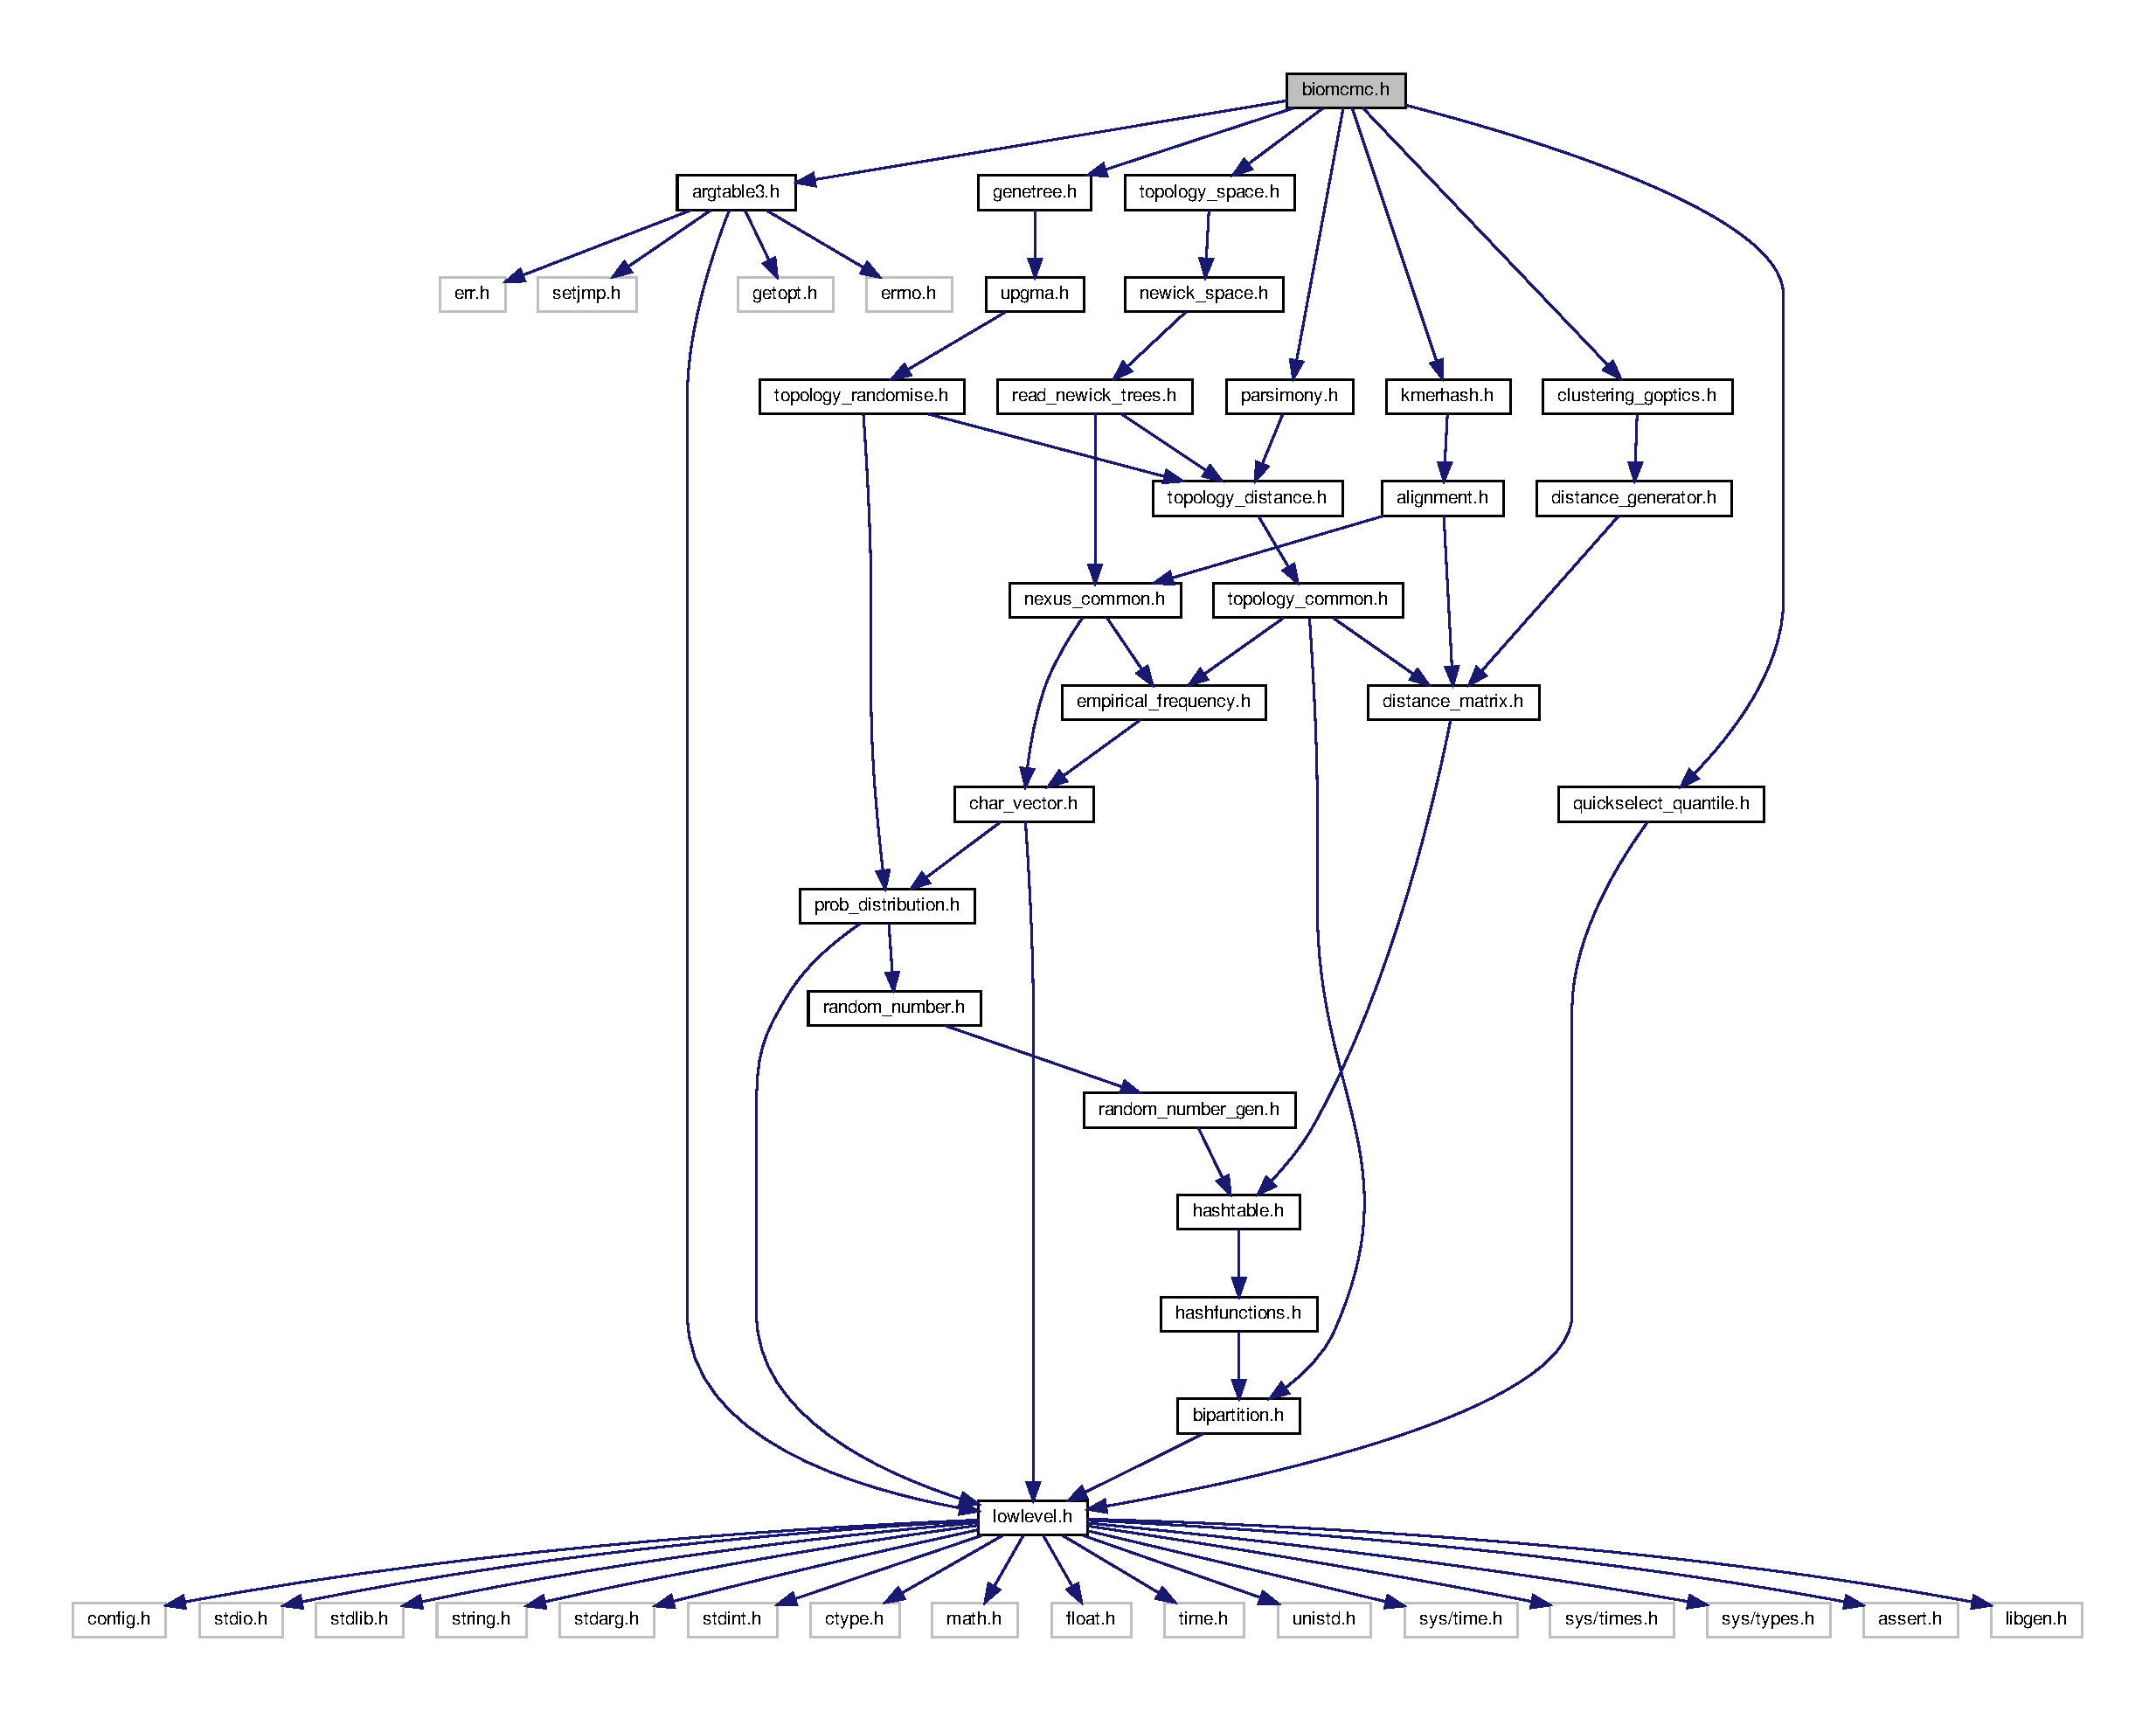
\includegraphics[width=350pt]{biomcmc_8h__incl}
\end{center}
\end{figure}


\subsubsection{Detailed Description}
biomcmc library interface to external programs, specific to super\+\_\+sptree repo. 

The idea is for biomcmc-\/lib is to be general for several sofware, including treesignal and super\+\_\+sptree. This library started branching from the biomcmc library from the guenomu software. It includes the edlib library for sequence pairwise edit distance (\href{http://martinsos.github.io/edlib}{\tt http\+://martinsos.\+github.\+io/edlib}) 